%%%%%%%%%%%%%%%%%%%%%%%%%%%%%%%%%%%%%%%%%%%%%%%%%%%%%%%%%%%%%%%%%%%%%
%% This is a (brief) model paper using the achemso class
%% The document class accepts keyval options, which should include
%% the target journal and optionally the manuscript type. 
%%%%%%%%%%%%%%%%%%%%%%%%%%%%%%%%%%%%%%%%%%%%%%%%%%%%%%%%%%%%%%%%%%%%%
\documentclass[journal=jacsat,manuscript=article]{achemso}

%%%%%%%%%%%%%%%%%%%%%%%%%%%%%%%%%%%%%%%%%%%%%%%%%%%%%%%%%%%%%%%%%%%%%
%% Place any additional packages needed here.  Only include packages
%% which are essential, to avoid problems later. Do NOT use any
%% packages which require e-TeX (for example etoolbox): the e-TeX
%% extensions are not currently available on the ACS conversion
%% servers.
%%%%%%%%%%%%%%%%%%%%%%%%%%%%%%%%%%%%%%%%%%%%%%%%%%%%%%%%%%%%%%%%%%%%%
\usepackage[version=3]{mhchem} % Formula subscripts using \ce{}

%%%%%%%%%%%%%%%%%%%%%%%%%%%%%%%%%%%%%%%%%%%%%%%%%%%%%%%%%%%%%%%%%%%%%
%% If issues arise when submitting your manuscript, you may want to
%% un-comment the next line.  This provides information on the
%% version of every file you have used.
%%%%%%%%%%%%%%%%%%%%%%%%%%%%%%%%%%%%%%%%%%%%%%%%%%%%%%%%%%%%%%%%%%%%%
%%\listfiles

%%%%%%%%%%%%%%%%%%%%%%%%%%%%%%%%%%%%%%%%%%%%%%%%%%%%%%%%%%%%%%%%%%%%%
%% Place any additional macros here.  Please use \newcommand* where
%% possible, and avoid layout-changing macros (which are not used
%% when typesetting).
%%%%%%%%%%%%%%%%%%%%%%%%%%%%%%%%%%%%%%%%%%%%%%%%%%%%%%%%%%%%%%%%%%%%%
\newcommand*\YE[1]{Ye: \texttt{\textbf{#1}}}

%%\newcommand{\YE}[1]{\textcolor{blue}{#1}}

%%%%%%%%%%%%%%%%%%%%%%%%%%%%%%%%%%%%%%%%%%%%%%%%%%%%%%%%%%%%%%%%%%%%%
%% Meta-data block
%% ---------------
%% Each author should be given as a separate \author command.
%%
%% Corresponding authors should have an e-mail given after the author
%% name as an \email command. Phone and fax numbers can be given
%% using \phone and \fax, respectively; this information is optional.
%%
%% The affiliation of authors is given after the authors; each
%% \affiliation command applies to all preceding authors not already
%% assigned an affiliation.
%%
%% The affiliation takes an option argument for the short name.  This
%% will typically be something like "University of Somewhere".
%%
%% The \altaffiliation macro should be used for new address, etc.
%% On the other hand, \alsoaffiliation is used on a per author basis
%% when authors are associated with multiple institutions.
%%%%%%%%%%%%%%%%%%%%%%%%%%%%%%%%%%%%%%%%%%%%%%%%%%%%%%%%%%%%%%%%%%%%%
\author{Ye Ding}
\affiliation{Atombeat Technology Pte. Ltd., 6 Rafflesr Quay, Singapore.}
\email{ye.ding@atombeat.com}
\author{Xinyan Wang}
\affiliation{Atombeat Technology Pte. Ltd., 6 Rafflesr Quay, Singapore.}
\email{xinyan.wang@atombeat.com}
\author{Rongfeng Zou}
\affiliation{Atombeat Technology Pte. Ltd., 6 Rafflesr Quay, Singapore.}
\author{Hang Zheng}
\affiliation{Atombeat Technology Pte. Ltd., 6 Rafflesr Quay, Singapore.}
\email{hzheng@atombeat.com}
%%%%%%%%%%%%%%%%%%%%%%%%%%%%%%%%%%%%%%%%%%%%%%%%%%%%%%%%%%%%%%%%%%%%%
%% The document title should be given as usual. Some journals require
%% a running title from the author: this should be supplied as an
%% optional argument to \title.
%%%%%%%%%%%%%%%%%%%%%%%%%%%%%%%%%%%%%%%%%%%%%%%%%%%%%%%%%%%%%%%%%%%%%
\title[An \textsf{achemso} demo]
  {Improving binding free energy predictions with Swap Monte Carlo for water sampling}

%%%%%%%%%%%%%%%%%%%%%%%%%%%%%%%%%%%%%%%%%%%%%%%%%%%%%%%%%%%%%%%%%%%%%
%% Some journals require a list of abbreviations or keywords to be
%% supplied. These should be set up here, and will be printed after
%% the title and author information, if needed.
%%%%%%%%%%%%%%%%%%%%%%%%%%%%%%%%%%%%%%%%%%%%%%%%%%%%%%%%%%%%%%%%%%%%%
\abbreviations{Free Energy Perturbation, Binding Free Energy, Monte Carlo, Water Sampling, Molecular Dynamics}
\keywords{American Chemical Society, \LaTeX}

%%%%%%%%%%%%%%%%%%%%%%%%%%%%%%%%%%%%%%%%%%%%%%%%%%%%%%%%%%%%%%%%%%%%%
%% The manuscript does not need to include \maketitle, which is
%% executed automatically.
%%%%%%%%%%%%%%%%%%%%%%%%%%%%%%%%%%%%%%%%%%%%%%%%%%%%%%%%%%%%%%%%%%%%%
\begin{document}

%%%%%%%%%%%%%%%%%%%%%%%%%%%%%%%%%%%%%%%%%%%%%%%%%%%%%%%%%%%%%%%%%%%%%
%% The "tocentry" environment can be used to create an entry for the
%% graphical table of contents. It is given here as some journals
%% require that it is printed as part of the abstract page. It will
%% be automatically moved as appropriate.
%%%%%%%%%%%%%%%%%%%%%%%%%%%%%%%%%%%%%%%%%%%%%%%%%%%%%%%%%%%%%%%%%%%%%
%\begin{tocentry}

%Some journals require a graphical entry for the Table of Contents.
%This should be laid out ``print ready'' so that the sizing of the
%text is correct.

%Inside the \texttt{tocentry} environment, the font used is Helvetica
%8\,pt, as required by \emph{Journal of the American Chemical
%Society}.

%The surrounding frame is 9\,cm by 3.5\,cm, which is the maximum
%permitted for  \emph{Journal of the American Chemical Society}
%graphical table of content entries. The box will not resize if the
%content is too big: instead it will overflow the edge of the box.

%This box and the associated title will always be printed on a
%separate page at the end of the document.

%\end{tocentry}

%%%%%%%%%%%%%%%%%%%%%%%%%%%%%%%%%%%%%%%%%%%%%%%%%%%%%%%%%%%%%%%%%%%%%
%% The abstract environment will automatically gobble the contents
%% if an abstract is not used by the target journal.
%%%%%%%%%%%%%%%%%%%%%%%%%%%%%%%%%%%%%%%%%%%%%%%%%%%%%%%%%%%%%%%%%%%%%
\begin{abstract}
Water molecules located within and surrounding the binding cavity can substantially affect ligand binding affinity.
Proper sampling of these water molecules ensures that their contributions to the free energy landscape are accurately accounted for. 
In the pursuit of more accurate binding free energy calculations, we have developed a novel Swap Monte Carlo (SwapMC) method specifically designed for cavity water sampling. 
The SwapMC method aims to enhance the sampling efficiency by facilitating the movement of water molecules in and out of the protein cavity, 
thereby ensuring a comprehensive exploration of water distributions. 
By leveraging GPU power to perform Monte Carlo moves for water molecules in parallel across multiple sites, 
and integrating SwapMC with NPT simulations within the Uni-FEP framework, 
we have observed significant improvements in the accuracy of relative binding free energy calculations, all while maintaining computational efficiency. 
Our results demonstrate that SwapMC achieves performance comparable to Grand Canonical Monte Carlo (GCMC) methods in water-related test cases, 
offering a robust and efficient alternative for addressing the challenges associated with cavity water sampling in molecular dynamics. 
%Furthermore, we have extended the SwapMC scheme to sample the distribution of ions in DNA/RNA simulations, 
%broadening the applicability of this method to a wider range of biomolecular systems and enhancing the accuracy of ion-related free energy calculations.
\end{abstract}

%%%%%%%%%%%%%%%%%%%%%%%%%%%%%%%%%%%%%%%%%%%%%%%%%%%%%%%%%%%%%%%%%%%%%
%% Start the main part of the manuscript here.
%%%%%%%%%%%%%%%%%%%%%%%%%%%%%%%%%%%%%%%%%%%%%%%%%%%%%%%%%%%%%%%%%%%%%
\section{Introduction}
Water molecules located within and surrounding the binding cavity substantially affect ligand binding affinity and selectivity through multiple distinct mechanisms~\cite{schiebel2018intriguing}. 
The multifaceted role of water in biomolecular recognition encompasses desolvation effects, where displacement of unfavorable water molecules from binding pockets drives binding through both enthalpic and entropic gains; 
water-mediated interactions, where conserved water molecules stabilize protein-ligand complexes through bridging hydrogen bond networks that can modulate binding affinity by over 1000-fold~\cite{darby2019water}; 
and first-shell hydration stabilization around solvent-exposed ligand moieties that contributes to binding thermodynamics~\cite{mahmoud2020elucidating, wang2011ligand}. 
The displacement of structurally constrained water molecules into bulk solvent results in significant entropic gains~\cite{cui2018role, portman2014enthalpy}, 
while approximately 80\% of water molecules bridging protein-ligand interfaces form three or more hydrogen bonds, 
highlighting their critical role in molecular recognition~\cite{poornima1995hydration}. 
These water-mediated interactions enable binding geometries that would be incompatible through direct protein-ligand contacts alone, 
underscoring that accurate computational treatment of water molecules is essential for predicting binding affinity~\cite{baron2010water,zsido2021role, maurer2019water}. \\
\newline
Binding free energy calculation for protein-ligand interactions has emerged as a transformative tool in computational chemistry and drug discovery~\cite{jiang2010free, wang2019protein, Qian2024}. 
Free energy perturbation (FEP) methods provide a thermodynamically rigorous framework for predicting binding affinities and are increasingly utilized in structure-based drug design to optimize ligand selectivity and potency~\cite{venkatesh2026evaluating, wang2019protein}. 
Recent benchmarks demonstrate that relative binding free energy (RBFE) calculations consistently achieve chemical accuracy ($\leq$~1 kcal/mol) in prospective drug discovery applications when properly executed~\cite{ross2023maximal}. 
FEP calculations can be categorized into two types: RBFE calculations where ligands are alchemically transformed between states in the binding site, 
and absolute binding free energy (ABFE) calculations where ligands are decoupled from the protein cavity. 
The accuracy of binding free energy calculations depends critically on two factors: force field parameters~\cite{Ding2023, 17c36m, lu2021opls4, he2022recent, vanommeslaeghe2012automationI, vanommeslaeghe2012automationII} and conformational sampling~\cite{15rex, wang2011replica, hritz2008hamiltonian}. 
Recent advances in force field development, including OPLS4~\cite{lu2021opls4}, CGenFF~\cite{vanommeslaeghe2012automationI, vanommeslaeghe2012automationII}, and GAFF2~\cite{he2022recent}, have substantially improved molecular representation accuracy, 
yet inadequate sampling of conformational space—particularly concerning water molecule distributions in binding sites—remains a significant bottleneck limiting FEP reliability and domain of applicability~\cite{ross2020enhancing}. \\
\newline
The sampling challenge is particularly acute for water molecules in protein binding sites, 
as conventional molecular dynamics simulations face severe kinetic bottlenecks in equilibrating buried water distributions~\cite{ross2020enhancing, BenShalom2019, ben2021fast}. 
Water exchange between buried cavities and bulk solvent occurs on microsecond timescales—well beyond typical FEP simulation lengths—creating a fundamental disconnection between fast local dynamics and slow water exchange processes~\cite{persson2008cell, kaieda2013internal}. 
During alchemical transformations, perturbations to the ligand structure frequently alter the optimal water distribution in the binding pocket, 
requiring accurate sampling of water occupancy at multiple sites~\cite{zhou2009theory, cozzini2004free,li2007water}. 
When water molecules cannot equilibrate on the simulation timescale, 
FEP calculations yield systematically biased free energy estimates with errors exceeding 5 kcal/mol—far larger than typical differences between structurally related compounds in lead optimization~\cite{ross2020enhancing}. 
The magnitude of this problem scales with binding site topology: solvent-exposed sites show minimal impact from sampling limitations, 
while deeply buried cavities with constricted access channels exhibit severe convergence problems. 
This sampling limitation has been recognized as a primary barrier to expanding FEP calculations to more challenging protein-ligand systems in drug discovery. \\
\newline
Multiple strategies have been proposed to enhance water sampling in binding sites~\cite{Wagle2024,ross2020enhancing,Ge2022,ben2021fast,Deng2024,Liu2025}. 
Grand Canonical Monte Carlo (GCMC) enables insertion and deletion of water molecules during MD simulations, 
with acceptance determined by the Metropolis criterion based on chemical potential~\cite{ross2015water, ross2020enhancing, Aldeghi2018, Bodnarchuk2014, deng2008computation, Samways2020, Woo2004}, 
and has demonstrated substantial improvements in FEP accuracy, reducing prediction errors from $<$3 kcal/mol to $<$1.5 kcal/mol for systems with water displacement~\cite{ross2020enhancing}.
Grand Canonical Nonequilibrium Candidate Monte Carlo (GCNCMC) combines GCMC with nonequilibrium dynamics to improve acceptance rates, achieving 5-10 times higher acceptance than standard GCMC while maintaining detailed balance~\cite{Bergazin2020,Ge2022,melling2023enhanced,Deng2024}. 
Grid Inhomogeneous Solvation Theory (GIST) computes spatially resolved solvation thermodynamics on a 3D grid to characterize favorable and unfavorable water positions~\cite{Abel2008,Michel2009,Cao2019,Irwin2019,Eberhardt2023}, 
while WaterMap clusters high-occupancy hydration sites and computes their thermodynamic contributions to binding~\cite{wang2011ligand}. 
Hybrid Monte Carlo/Molecular Dynamics methods supplement standard MD with translational MC moves for water molecules without requiring chemical potential determination or handling variable particle numbers~\cite{BenShalom2019,ben2021fast}. 
However, these methods face common limitations: GCMC and GCNCMC require system-dependent chemical potential calibration; 
GIST and WaterMap characterize existing water distributions but do not directly accelerate sampling during alchemical transformations; 
and most molecular dynamics engines lack native implementations of these techniques~\cite{Samways2020,Cezar2020,Nejahi2021,Nejahi2019}. 
These barriers have limited routine adoption despite demonstrated effectiveness, 
highlighting the need for alternative approaches that balance sampling efficiency, thermodynamic rigor, and practical accessibility.\\
\newline
In this work, we present Swap Monte Carlo (SwapMC), a novel method designed to efficiently sample water molecules in protein cavities during binding free energy calculations. 
SwapMC operates within the NPT ensemble, eliminating the need for chemical potential calibration required by GCMC methods. 
The method allows exchange of water molecules between the cavity and bulk solvent regions, 
with acceptance ratios derived from detailed balance conditions dependent only on interaction energies and regional volumes. 
By leveraging GPU parallelization to evaluate interaction energies for thousands of potential water insertion sites simultaneously, 
SwapMC achieves computational efficiency comparable to standard MD while dramatically enhancing water sampling. 
Implementation within the Uni-FEP framework using the OpenMM~\cite{Eastman2023} simulation engine provides seamless integration with existing FEP workflows without requiring specialized Monte Carlo packages or external tools. 
SwapMC thus addresses key barriers limiting adoption of advanced water sampling techniques: elimination of chemical potential tuning, compatibility with standard NPT simulations, natural integration into FEP protocols, and GPU-accelerated computational efficiency. \\
\newline
To validate the effectiveness of SwapMC, we conducted comprehensive tests on established benchmark sets comparing performance with GCMC and standard MD approaches~\cite{ross2020enhancing}. 
We begin by describing the SwapMC workflow in the Uni-FEP framework and deriving the acceptance ratio from detailed balance conditions. 
We then present the performance of SwapMC in both relative and absolute binding free energy calculations, 
demonstrate its ability to sample water distributions in protein cavities through analysis of contact water numbers, 
and show that SwapMC achieves comparable performance with GCMC. 
These results demonstrate that SwapMC provides an effective, accessible, and robust solution for incorporating proper water sampling into routine binding free energy calculations.
\section{Method}
The Swap Monte Carlo (SwapMC) method enhances water sampling in protein cavities by facilitating exchange of water molecules between the binding region and bulk solvent. 
Unlike Grand Canonical Monte Carlo (GCMC), which inserts or deletes water molecules, 
SwapMC maintains constant particle number within the NPT ensemble, 
thereby avoiding the need for chemical potential calibration. 
This section describes the algorithmic workflow, theoretical foundations ensuring detailed balance, 
and GPU-accelerated implementation within the Uni-FEP framework.

\subsection{Workflow of the Swap Monte Carlo}
The SwapMC algorithm facilitates water exchange between the cavity region and bulk solvent during FEP calculations, Fig.~\ref{fig:scheme} A.
The cavity region ($R^{in}$ in Fig.~\ref{fig:scheme} B) is defined as a spherical volume centered at the geometric centroid of the ligand heavy atoms, with radius $r_{cavity}$ calculated as: $r_{cavity} = \frac{1}{2} \cdot \max_{i,j} \parallel \mathbf{r_i} - \mathbf{r_j} \parallel + 0.3 \text{~nm}$,
where $r_i$ and $r_j$ denote positions of ligand heavy atoms $i$ and $j$. 
This buffer distance (0.3~nm) ensures inclusion of the first hydration shell beyond the ligand van der Waals surface. 
The exterior region ($R^{out}$ in Fig.~\ref{fig:scheme} B) comprises all simulation volume outside $R^{in}$.
This approach reduces computational overhead from MC moves on waters distant from the binding site, compared to the fixed rectangular regions employed by Ben-Shalom et al~\cite{ben2021fast}. \\
\newline
The SwapMC algorithm workflow consists of these steps:
\begin{enumerate}
  \item Randomly decide the exchange direction, ensuring an equal chance of moving water in or out of the cavity.
  \item Biased water selection. The algorithm selects a water molecule $i$ for deletion from the source region with probability $p_i$ given by Eq.~\ref{eq:selection_probability}. This Boltzmann-weighted selection biases toward waters with higher (less favorable) interaction energies $u_i$, 
  thereby increasing acceptance rates for swaps that replace unfavorable waters with potentially favorable configurations.
  Here, $N_{src}$ denotes the number of exchangeable water molecules in the source region ($R_{in}$ for cavity $\to$ bulk moves; $R_{out}$ for bulk $\to$ cavity moves). 
  The selection probabilities are normalized such that $\sum_{k} p_k$ = 1.
  \begin{equation}\label{eq:selection_probability}
    p_i = \frac{e^{u_i}}{\sum^{N_{src}}_k{e^{u_k}}}    
  \end{equation}
  %\item Uniform sampling the potential insertion sites over the destination region.
  \item Parallel energy evaluation. The combination of 300 uniformly sampled insertion sites with 60 water orientations yields 18,000 candidate insertion conformations per swap attempt. 
  Water orientations were sampled using 60 approximately uniformly distributed unit quaternions~\cite{karney2007quaternions}, providing systematic coverage of the rotation group SO(3).
  Interaction energies $u_j$ for all candidate conformations are evaluated in parallel on GPUs using our custom OpenMM nonbonded interaction module, enabling efficient exploration of the insertion phase space within milliseconds per swap attempt.
  \item The potential insertion conformations are sequentially evaluated. 
  For each conformation, the acceptance ratio $A_{S_i \to S_j}$ is calculated according to Eq.~\ref{eq:acceptance_ratio}. 
  The first conformation to satisfy the Metropolis criterion (random number  $< A_{S_i \to S_j}$) is accepted, and the iteration proceeds to Step 5.
  \item Atomic coordinates of the deleted water molecule are updated to match the accepted conformation. 
  The velocity vector of this water molecule is reset to zero to maintain numerical stability in the subsequent MD steps.
\end{enumerate}

\begin{figure}
  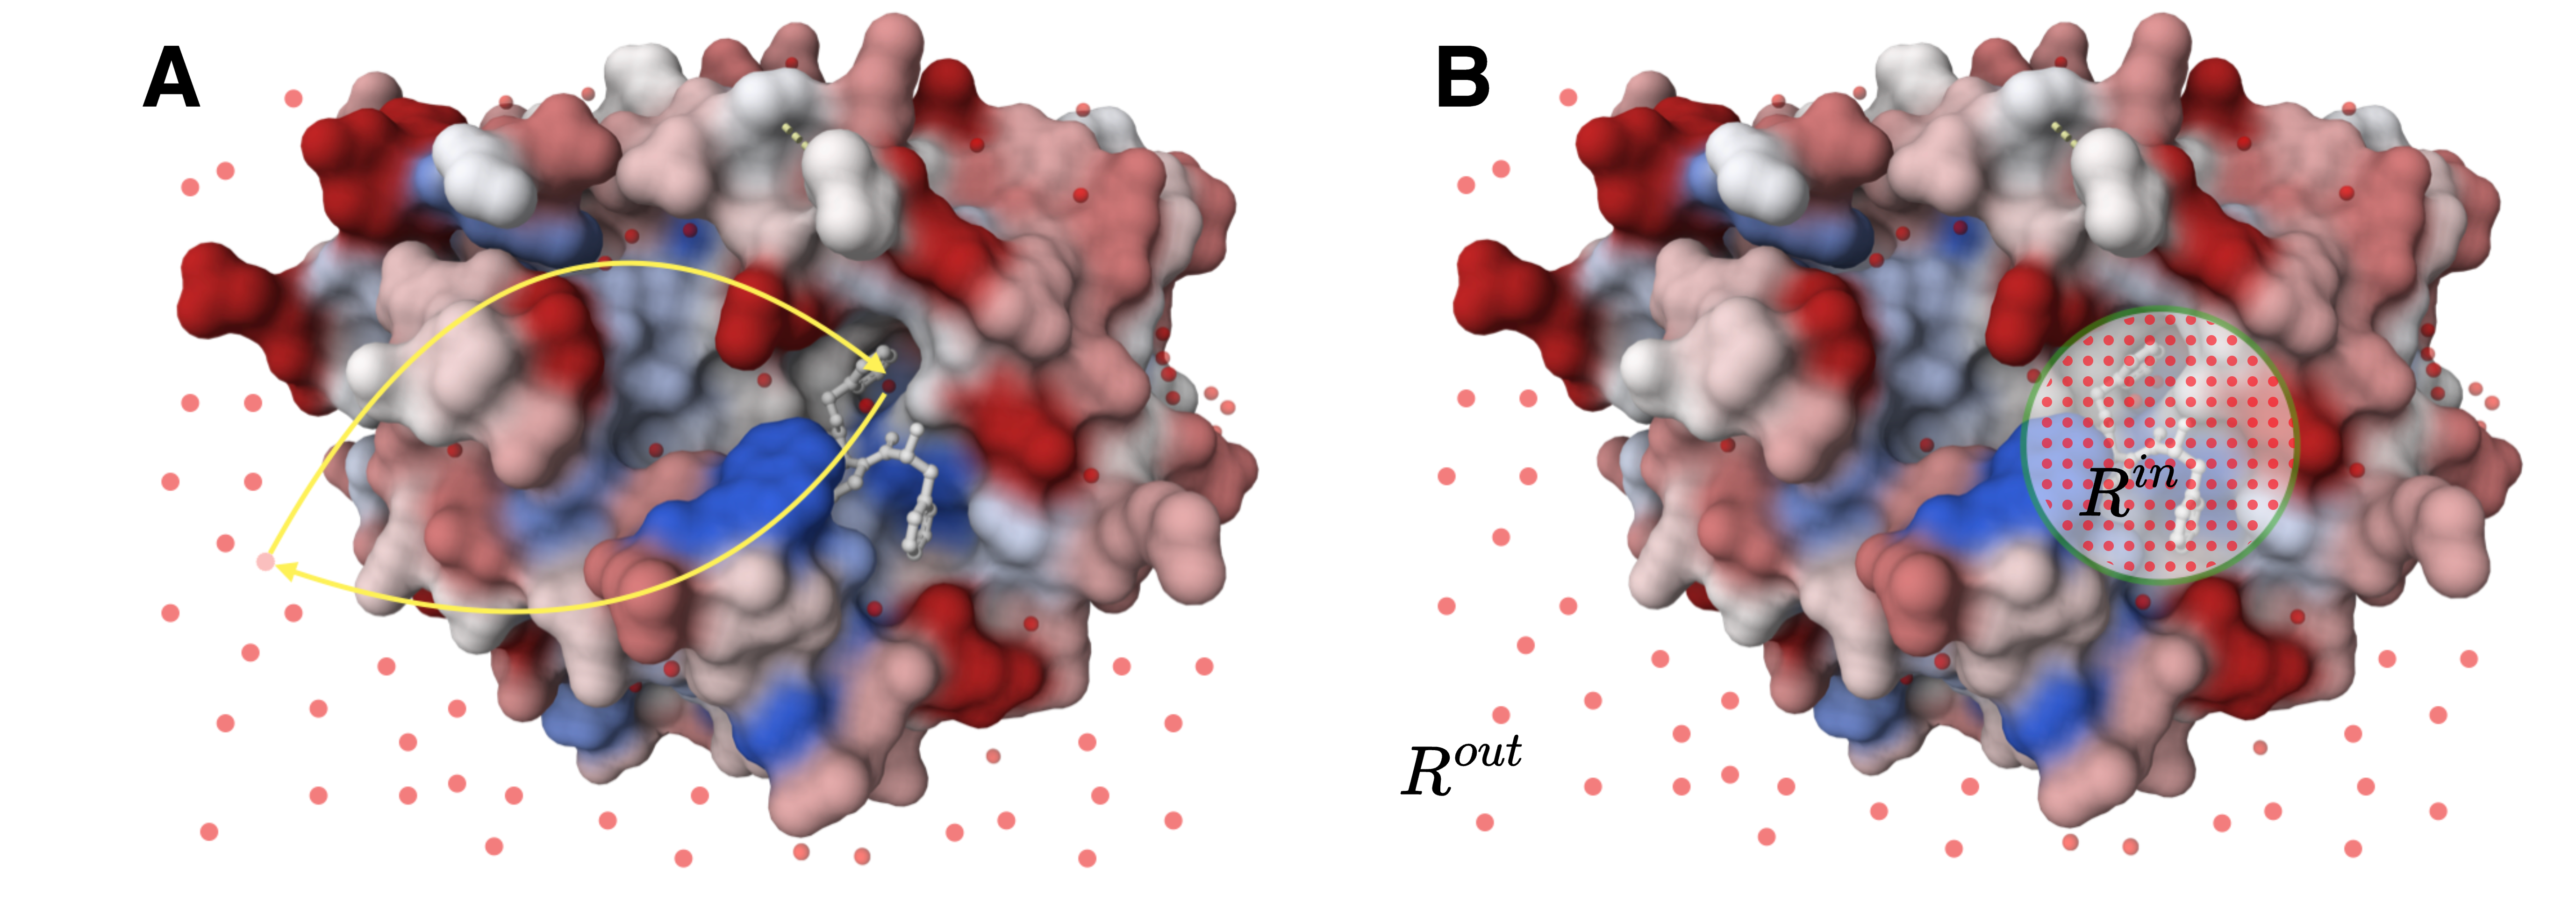
\includegraphics[width=0.9\textwidth]{figures/SwapMonteCarlo-scheme.png}
  \caption{Schematic Figure for Swap Monte Carlo (SwapMC) Method.
  The figure illustrates the process of exchanging water molecules between the cavity region and bulk solvent during simulation.}
  \label{fig:scheme}
\end{figure}

\subsection{Detailed Balance in Swap Monte Carlo}
To ensure SwapMC samples the correct canonical (NPT) ensemble, 
the acceptance criterion must satisfy detailed balance—a fundamental requirement guaranteeing that the equilibrium distribution is a stationary solution of the Markov chain. 
We derive the acceptance ratio $A_{S_i \to S_j}$ by requiring microscopic reversibility between states $S_i$ and $S_j$, 
which differ only in the position of a single water molecule while all other atoms remain fixed. \\
\newline
In the Monte Carlo algorithm, the acceptance ratio $A_{S_i \to S_j}$ between two states $S_i$ and $S_j$ must satisfy detailed balance:
\begin{equation}\label{eq:acceptance_ratio}
\frac{A_{S_i \to S_j}}{A_{S_j \to S_i}}=\frac{G_{S_j \to S_i} P_{S_j}}{G_{S_i \to S_j} P_{S_i}}
\end{equation}
\noindent Where $P_{S_j}$ and $P_{S_i}$ represent the equilibrium probabilities of states $S_j$ and $S_i$, respectively. 
The terms $G_{S_i \to S_j}$ and $G_{S_j \to S_i}$ denote the transition probabilities for the transformation from state $S_i$ to state $S_j$, and vice versa.
As the Metropolis criteria indicated, in simulations, the acceptance ratio $A_{S_i \to S_j}$ for the transformation from state $S_i$ to $S_j$, is defined as:
\begin{equation}\label{eq:metropolis}
A_{S_i \to S_j}=\min \left\{1, \frac{G_{S_j \to S_i} P_{S_j}}{G_{S_i \to S_j} P_{S_i}}\right\}
\end{equation} 
In the context of Swap Monte Carlo, state $S_i$ represent the water molecule located in position $\mathbf{x}_i$, and state $S_j$ represents the water molecule located in position $\mathbf{x}_j$, where the other atoms remains fixed.
In the canonical (NPT) ensemble at fixed particle number $n$, the equilibrium probability of a microstate follows the Boltzmann distribution. 
For states $S_i$ and $S_j$ differing only in a water molecule position:
\begin{equation}\label{eq:equilibrium_probability}
  \begin{aligned}
  P_{S_i}\left(\mathbf{x}_1, \ldots, \mathbf{x}_i, \ldots\mathbf{x}_n\right) & \propto \frac{1}{n!} e^{-\beta U\left(\mathbf{x}_1, \ldots, \mathbf{x}_i,\ldots, \mathbf{x}_n\right)}  \\
  P_{S_j}\left(\mathbf{x}_1, \ldots, \mathbf{x}_j, \ldots\mathbf{x}_n\right) & \propto \frac{1}{n!} e^{-\beta U\left(\mathbf{x}_1, \ldots, \mathbf{x}_j,\ldots, \mathbf{x}_n\right)}
  \end{aligned}
\end{equation} 
where the factor $1/n!$ accounts for indistinguishability of identical water molecules, 
$ \beta = 1/k_B T $ is the inverse temperature, $k_B$ is Boltzmann's constant. 
The $n!$ terms cancel when computing probability ratios, simplifying the acceptance criterion derivation.
And $U\left(\mathbf{x}_1, \ldots, \mathbf{x}_i,\ldots, \mathbf{x}_n\right)$, $U\left(\mathbf{x}_1, \ldots, \mathbf{x}_j,\ldots, \mathbf{x}_n\right)$ denotes the potential energy of the states $S_i, S_j$.
%$\beta = \frac{1}{kT}$ is the inverse temperature, $k$ is the Boltzmann constant, and $n$ is the number of particles in the system.
A fundamental relationship emerges from the potential energy difference between two states $S_i$ and $S_j$:
\begin{equation}\label{eq:potential_energy_interaction}
U\left(\mathbf{x}_1, \ldots, \mathbf{x}_j,\ldots, \mathbf{x}_n\right) - U\left(\mathbf{x}_1, \ldots, \mathbf{x}_i,\ldots, \mathbf{x}_n\right) = u_j - u_i
\end{equation}
Where $u_i$ and $u_j$ are the interaction energies of the moved water molecule in states $S_i$ and $S_j$, respectively.
\newline
The transition probability matrix element $G_{S_i \to S_j}$ quantifies the likelihood of transitioning from state $S_i$ to state $S_j$. 
Given the statistical independence between molecular deletion and insertion events, 
the composite transition probability necessarily factorizes as:
\begin{equation}\label{eq:transition_probability_decomposition}
G_{S_i \to S_j} = g_{S_i}^{(\text{del})} \cdot g_{S_j}^{(\text{ins})}
\end{equation}
Where $g_{S_i}^{(\text{del})}$ and $g_{S_j}^{(\text{ins})}$ represent the respective marginal probabilities for water molecule removal from state $S_i$ and insertion into state $S_j$.
With the previous workflow steps, the deletion probability $g_{S_i}^{(\text{del})}$ is defined as the probability of selecting a water molecule $i$ for deletion from the source region, 
given by Eq.~\ref{eq:selection_probability}, 
and the insertion probability $g_{S_j}^{(\text{ins})}$ is defined as the uniform sampling of the potential insertion sites over the destination region.
Thus, the transformation probability matrix elements $G_{S_i \to S_j}$ and $G_{S_j \to S_i}$ can be expressed as:
\begin{equation}\label{eq:transition_probability}
  \begin{aligned}
G_{S_i \to S_j} &= p_i \cdot \frac{1}{V_{S_j}} = \frac{e^{u_i}}{\sum^{N^{S_i}_{src}}_k{e^{u_k}}} \cdot \frac{1}{V_{S_j}} \\
G_{S_j \to S_i} &= p_j \cdot \frac{1}{V_{S_i}} = \frac{e^{u_j}}{\sum^{N^{S_j}_{src}}_k{e^{u_k}}} \cdot \frac{1}{V_{S_i}}  
  \end{aligned}
\end{equation}
Where $V_{S_i}$ and $V_{S_j}$ denote the volume of the source region in states $S_i$ and $S_j$, respectively.
%Critical asymmetry in source regions. 
The cardinalities $N_{\text{src}}^{S_i}$ and $N_{\text{src}}^{S_j}$ differ because the source regions for forward ($S_i \to S_j$) and reverse ($S_j \to S_i$) transformations are complementary. 
For a cavity$\to$bulk move ($x_i \in R^{in}$, $x_j \in R^{out}$): \\
Forward source region: $$N^{S_i}_{\text{src}} = |\text{waters in } R^{in}|$$ \\
Reverse source region: $$N^{S_j}_{\text{src}} = |\text{waters in } R^{out}| + 1$$ \\
The "+1" accounts for the newly placed water at $x_j$, which becomes eligible for selection in the reverse move. 
This asymmetry is essential for satisfying detailed balance and is reflected in the ratio of partition functions in Eq.~\ref{eq:acceptance_criterion}. \\
\newline
%The source region cardinalities $N_{\text{src}}^{S_i}$ and $N_{\text{src}}^{S_j}$ in the transition probability elements $G_{S_i \to S_j}$ and $G_{S_j \to S_i}$ correspond to distinct spatial domains within the simulation framework, 
%as their respective source regions differ between the transformation $S_i \to S_j$ and $S_j \to S_i$.
%Assume the position $\mathbf{x}_i$ is within the cavity region $R^{in}$, and the position $\mathbf{x}_j$ is outside the cavity region $R^{out}$.
%The source region $N_{\text{src}}^{S_i}$ is defined as the set of water molecules within the cavity region $R^{in}$, 
%and the source region $N_{\text{src}}^{S_j}$ is defined as the set of water molecules outside the cavity region $R^{out}$ plus the moved water molecule in position $\textbf{x}_j$. \\
%To formally distinguish these non-overlapping regions, we employ the notation $N_{\text{src}}^{S_i}$ and $N_{\text{src}}^{S_j}$ as domain-specific particle counts.
By substitute the components in Eq.~\ref{eq:metropolis} with the Eq.~\ref{eq:equilibrium_probability},~\ref{eq:potential_energy_interaction},~\ref{eq:transition_probability},
we obtained the acceptance criterion for the exchange of water molecules in transition $S_i \to S_j$:
\begin{equation}\label{eq:acceptance_criterion}
A_{S_i \to S_j} = \min \left\{1, \frac{V_{S_j}}{V_{S_i}} \cdot \frac{\sum^{N^{S_i}_{src}}_k{e^{u_k}}}{\sum^{N^{S_j}_{src}}_k{e^{u_k}}} \right\}
\end{equation}
\noindent The acceptance criterion required the calculations on the interaction energies $u_k$ of all water molecules in the source region $N^{S_i}_{src}$ or $N^{S_j}_{src}$,
which can be efficiently performed in parallel on GPUs.
\subsection{Implementation of Swap Monte Carlo in OpenMM}
The SwapMC method was implemented within the Uni-FEP framework built upon OpenMM~\cite{Eastman2023}, 
leveraging GPU acceleration for efficient water sampling. 
We rewrote OpenMM's nonbonded interaction module to compute per-water interaction energies in parallel, 
evaluating all water molecules in simulation system across GPU threads simultaneously. 
A critical optimization leverages OpenMM's native neighbor list infrastructure, which is automatically maintained during MD simulation. 
Rather than recomputing pair distances, SwapMC inherits this precomputed neighbor list, reducing energy evaluation cost for water-protein interactions by restricting calculations to relevant atoms instead of the full system. 
Long-range electrostatics in interaction energies are computed using the Reaction-Field method ($\epsilon = 80$) to approximate PME interactions while enabling fully GPU-local computation without global FFT operations. \\
\newline 
Water molecule selection from the source region employs the Gumbel-Max Trick for GPU compatibility~\cite{huijben2022review}. 
This method enables direct parallel sampling by computing log-probabilities and Gumbel noise independently for each water molecule, 
then selecting via parallel max-reduction in $O(\log N_{\text{src}})$ time. 
This approach avoids the serial bottleneck of computing cumulative probabilities and sorting, which would severely limit GPU utilization, 
while remaining theoretically equivalent to rejection-free sampling from the categorical distribution defined by the biased selection probabilities. \\
\newline
Following water selection, the method evaluates 18,000 candidate insertion conformations in parallel using the optimized nonbonded module. 
Each GPU thread computes the interaction energy $u_j$ for one candidate conformation, with data cached in GPU shared memory for efficiency.
The first conformation satisfying the Metropolis criterion is immediately accepted, terminating the screening loop for that swap attempt.
This sequential-acceptance strategy maintains detailed balance while ensuring computational efficiency, 
as finding one acceptable candidate quickly is more efficient than exhaustively scoring all 18,000 candidates. \\
\newline
These GPU optimizations enable practical SwapMC sampling for production FEP calculations. 
Each swap attempt requires ~2 milliseconds on NVIDIA 4090 GPUs (50,000-atom systems, 300 insertion sites). 
With SwapMC attempts every 1000 MD steps (4 ps with a 4 fs timestep), the simulation throughput decreases by less than 5\% compared to 
standard MD—a modest overhead that is easily justified by the substantial improvements in water sampling and binding free energy accuracy demonstrated in the Results.

\section{Results}
To validate the SwapMC method, we evaluated its performance on two complementary benchmark sets: 
(1) the "water sets" from Ross et al.~\cite{ross2020enhancing}, comprising 94 ligand transformations across 8 protein systems where water displacement significantly impacts binding affinity; 
and (2) the JACS set of 8 diverse protein targets for absolute binding free energy calculations. 
These benchmarks were specifically chosen because poor water sampling has been identified as a primary source of error in conventional FEP calculations for these systems~\cite{ross2020enhancing, Liu2025, luccarelli2010effects, Ge2022}. \\
\newline
Our validation strategy progresses through three stages: 
(1) demonstrating that SwapMC accelerates water equilibration through direct sampling analysis, 
(2) evaluating RBFE accuracy and comparing with GCMC benchmarks, including robustness assessment across different initial water configurations, 
and (3) extending validation to ABFE calculations. 
%All calculations utilized identical benchmark systems, transformations, and experimental data as Ross et al. for rigorous comparison.
For direct comparison with GCMC, we utilized identical protein systems, alchemical transformation edges, and experimental reference data as Ross et al~\cite{ross2020enhancing}. \\
\newline
%For a robust validation of the Swap Monte Carlo method, 
%we conducted a series of tests to evaluate its performance in free energy calculations.
%Gregory et.al~\cite{ross2020enhancing} performed a comprehensive evaluation of the GCMC method for water sampling in the RBFE calculations.
%The test set in Gregory's work includes 94 ligands in 8 diverse protein-ligand systems.
%For each system, the transformation of the ligands in RBFE calculations is related to the water displacement in the protein cavity.
%GCMC has been shown to be effective in sampling water molecules in the protein cavity~\cite{ross2015water},
%and showed a significant improvement in the accuracy of RBFE calculations compared to the traditional MD simulations for RBFE with water displacement transformation.
%In this work, we made a direct comparison of the performance of SwapMC with GCMC in the same test cases.
YE: Add more details about the RBFE and ABFE tests. Such as the mapping, lambda schedule, etc.

All tests were performed with the Uni-FEP framework.
RBFE simulations were performed with the Uni-FEP framework, 
each replica was run for 5~\textit{ns} with a time step of 4~\textit{fs}.
SwapMC was performed every 1000 steps (4~\textit{ps}) during the simulation.
300 potential insertion sites were uniformly sampled in the cavity region for each replica.
TIP3P~\cite{Jorgensen1983} water model was used in all simulations.
Ligands parameterization was performed with GAFF2~\cite{he2020fast} and ff14SB~\cite{Maier2015} was used for protein force field.


\subsection{Water Sampling in Protein Cavity}
To illustrate SwapMC's water sampling capabilities, we examined the alchemical transformation of Ligand 9 to Ligand 7 within the HSP90 binding site (Fig. 2A), 
a perturbation involving core scaffold hopping that fundamentally alters the cavity water network. 
This transformation serves as a stringent test case because the structural rearrangement induces subtle but thermodynamically significant changes in water distribution that conventional MD fails to capture, 
particularly when initial structures lack pre-equilibrated water molecules. \\
\newline
To create a challenging sampling scenario, we removed all water molecules from the cavity region in the initial structure, 
requiring the simulation to repopulate the hydration network from bulk solvent. 
Contact water molecules were defined as waters with oxygen atoms within 5~\AA~of heavy atoms in the perturbed ligand regions, 
providing a sensitive metric for cavity hydration state. 
Fig.~\ref{fig:hsp90} B tracks the evolution of contact water numbers across 24~$\lambda$-windows during the 5~\textit{ns} production phase for each replica. \\
\newline
Without SwapMC, contact water numbers remained suppressed throughout the transformation, 
particularly at intermediate $\lambda$-values ($5 < \lambda < 18$) where structural changes are most substantial. 
This indicates incomplete water equilibration on the 5 ns timescale, consistent with microsecond-scale water exchange kinetics in buried cavities. % Shall we recheck this number? 
In contrast, SwapMC-enabled simulations rapidly repopulated the cavity, 
achieving near-equilibrium contact water numbers within the first nanosecond and maintaining stable populations thereafter. \\
\newline
The differential water occupancy between ligand endpoints reflects chemical intuition: 
Ligand 7 accommodates 4.1 ± 0.5 contact waters compared to 2.3 ± 0.4 for Ligand 9, 
a 78\% increase consistent with the additional hydroxyl group in Ligand 7 that stabilizes bridging interactions to protein residues. 
Standard MD without enhanced sampling failed to equilibrate this water network, yielding artificially low contact water populations and consequently systematic underestimation of solvation contributions to binding affinity. \\
\newline
The improved water sampling directly translated to substantial gains in thermodynamic accuracy. 
For the Ligand 9→7 transformation, SwapMC reduced the error in ΔΔG_bind from 4.82 ± 0.71 kcal/mol (no SwapMC) to 0.23 ± 0.68 kcal/mol (with SwapMC) compared to the experimental value of -2.1 kcal/mol (Table S3). 
This 4.59 kcal/mol improvement demonstrating that inadequate water sampling was the dominant source of error for this transformation.


For a more intuitive understanding of the water displacement in the protein cavity, 
we have selected two ligands from the HSP90 protein-ligand system, Ligand 9 and Ligand 7, as shown in Fig.~\ref{fig:hsp90} A.
The transformation of Ligand 9 to Ligand 7 involves the core hopping change of the two ligands,
which results in a subtle water distribution change in the protein cavity.
However, the change of the water distribution in the cavity is hard to be captured by the traditional MD simulations.
Especially for the structures without pre-equilibration, the water molecules in the cavity region are not well sampled.\\
\newline
In this test, the alchemical transformation was performed between Ligand 9 to Ligand 7.
The water molecules in the cavity region were removed in the input structure of the simulation.
Fig.~\ref{fig:hsp90} B showed changes of the number of contact water molecules.
Number of contact water molecules is defined as the number of water molecules that are within 5~\textit{Å} from the heavy atoms of the alchemical changed group of the ligands.
In the cavity region with different replicas during the alchemical transformation.
Within the 5~\textit{ns} simulation for each replica,
the number of contact water molecules with SwapMC is significantly higher than that without SwapMC.
Ligand 7 has larger number of contact water molecules in the cavity region than Ligand 9,
which is consistent with the ligand structure change.
These results indicate that SwapMC made a more thorough sampling of the water molecules in the cavity region.
And it also captured the subtle change of the water distribution in the cavity region with distinct ligands.
With the SwapMC enabled, the RBFE results for the alchemical transformation of Ligand 9 to Ligand 7 is significantly improved 4.59~\textit{kcal/mol} compared to the results without SwapMC.
\begin{figure}
  \includegraphics[width=0.9\textwidth]{figures/hsp90.png}
  \caption{Water sampling in the HSP90 protein cavity in the presence of a ligand. 
  Panel A shows the two ligands (Ligand 9 and Ligand 7) used in the test.
  Panel B shows the number of contact water molecules in the cavity region during the alchemical transformation of Ligand 9 to Ligand 7.
  Replica 0 denotes the Ligand 9 state, and Replica 23 denotes the Ligand 7 state.
  }
  \label{fig:hsp90}
\end{figure}

\subsection{Performance on RBFE Calculations}
Water sampling was significantly improved with the SwapMC method.
That paved the way for the RBFE calculations with water displacement transformation.
We have performed the RBFE calculations on the water sets in Gregory's work~\cite{ross2020enhancing}.
For a fair comparison, we conducted four sets of RBFE calculations for each system:
With and without SwapMC, and with and without cavity waters (CW.).
Cavity waters are the crystal waters that located in the 6~\textit{Å} radius of the ligand heavy atoms.
All simulations were ran with the same protocol as described in the previous section.\\ 
\newline
The RBFE results are shown in Table~\ref{tbl:rbfe_watersets}.
Compared to the results without SwapMC, the RBFE results with SwapMC show a significant improvement in accuracy.
Besides, SwapMC showed a good consistency in the RBFE results with and without cavity waters in input structure.
Which indicates the robustness of the SwapMC method in water sampling.
Furthermore, the RBFE results with SwapMC are comparable to the GCMC results in these systems.
These results demonstrate that SwapMC can be an effective alternative to GCMC for water sampling in RBFE calculations.

\begin{table}
  \caption{RBFE results for water sets, where CW denotes Cavity Waters. All edges correspond to those utilized in Gregory's study~\cite{ross2020enhancing}. 
  The ddG RMSE and $R^2$ values are computed using experimental binding free energies. 
  The unit of ddG RMSE is \textit{kcal/mol}, with $R^2$ presented in parentheses. 
  The optimal results are highlighted in \textbf{bold}.}
  \label{tbl:rbfe_watersets}
  \begin{tabular}{l|lllll}
    \hline
    System                    & No CW.     & No CW.        & With CW.    & With CW.     & GCMC by  \\
    ddG RMSE ($R^2$)          & No SwapMC  & With SwapMC   & No SwapMC   & With SwapMC  & Gregory et al.~\cite{ross2020enhancing} \\
    \hline
    Brd4(1)                      & 1.34 (0.67) & 0.87 (0.82) & 1.07 (0.71) & \textbf{0.64 (0.93)} & 1.74 (0.01) \\
    Chk1                         & 2.99 (0.02) & 1.67 (0.43) & 2.64 (0.10) & 1.70 (0.47) & \textbf{0.78 (0.80)} \\
    HSP90\_Kung                  & 3.85 (0.11) & 1.51 (0.59) & 3.90 (0.16) & \textbf{1.50} (0.50) & 2.14 (\textbf{0.62}) \\
    HSP90\_Woodhead              & 2.27 (0.83) & 0.61 (0.98) & 2.25 (0.84) & 0.65 (0.97) & \textbf{0.26} (\textbf{1.00}) \\
    Scytalone                    & 2.25 (0.73) & 1.45 (0.84) & 1.90 (0.80) & \textbf{1.39 (0.85)} & 1.86 (0.77) \\
    Taf1(2)                      & 2.01 (0.08) & 0.70 (0.51) & 0.76 (0.34) & 0.66 (0.51) & \textbf{0.66 (0.78)} \\
    Thrombin                     & 1.37 (0.34) & 1.14 (0.64) & 1.20 (0.46) & \textbf{1.13 (0.66)} & 1.15 (0.49) \\
    Urokinase                    & 0.74 (0.62) & 0.91 (0.36) & 0.81 (0.52) & 0.94 (0.32) & \textbf{0.70 (0.74)} \\
    \hline
  \end{tabular}
\end{table}

\subsection{Performance on ABFE Calculations}
The performance of SwapMC was also evaluated in the absolute binding free energy (ABFE) calculations.
During the ABFE calculations, the decoupling of the ligand from the protein cavity requires the water molecules in the cavity to be well sampled.
Reorganization of the water molecules in the cavity region is crucial for the accurate calculation of the binding free energy.
Previous studies~\cite{Liu2025} have shown that enhancing the sampling of water molecules in the cavity region can improve the convergence of the ABFE calculations. \\
\newline
In this work, we have performed the ABFE calculations on the JACS set and compared the performance of SwapMC with the results ordinary MD simulations.
The ABFE calculations were performed with the same protocol as described in the previous section.
The JACS set consists of 8 protein-ligand systems, and the binding free energy calculations were performed with the Uni-FEP framework.
The results are shown in Table~\ref{tbl:abfe_jacs}.
Compared to the results without SwapMC, the ABFE results with SwapMC show a significant improvement in the accuracy of the binding free energy calculations.
Most of the systems show a significant reduction in the dG RMSE, and the $R^2$ values are also improved.

\begin{table}
  \caption{ABFE Results for JACS set with and without SwapMC.}
  \label{tbl:abfe_jacs}
  \begin{tabular}{l|ll}
    \hline
    System                    & No SwapMC     & With SwapMC    \\
    dG RMSE ($R^2$)           &               &    \\
    \hline
    BACE                      & 3.27 (0.25) & \textbf{2.68} (0.20)  \\
    CDK2                      & 3.99 (0.09) & \textbf{2.04} (0.55)  \\
    JNK1                      & 2.01 (0.48) & \textbf{0.77} (0.63)  \\
    MCL1                      & 2.05 (0.34) & \textbf{1.67} (0.36)  \\
    P38                       & 3.22 (0.31) & 3.25 (0.46) \\
    PTP1B                     & 8.78 (0.29) & \textbf{4.94} (0.33) \\
    Thrombin                  & 1.67 (0.35) & 1.82 (0.72) \\
    TYK2                      & 2.51 (0.40) & \textbf{1.35} (0.47) \\
    \hline
  \end{tabular}
\end{table}


\section{Conclusion and Discussion}
We present a novel Swap Monte Carlo (SwapMC) method designed to efficiently sample water molecules in the cavity during binding free energy calculations.
Compared with the traditional MD simulations, SwapMC significantly improves the sampling of water molecules in the cavity region.
By integrating SwapMC with the Uni-FEP framework, the binding free energy calculations gained a notable improvements under the NPT ensemble.
Further testing on the water sets in Gregory's work~\cite{ross2020enhancing} demonstrated that SwapMC achieves comparable performance with GCMC in binding free energy calculations. 
Without the tuning of the chemical potential in SwapMC makes it it easy to be extended to other FEP framework. 
We hope that our work can provide a robust and efficient alternative for addressing the challenges associated with cavity water sampling in computational chemistry. \\
\newline
Currently, SwapMC was only implemented for the water molecules in the protein cavity.
Extend the SwapMC method to sample the distribution of ions in DNA/RNA simulations is a promising direction for future work.
Furthermore, monte carlo methods can also be applied to sample the distribution of other small molecules in the binding site,
such as the ligand fragments or the co-factors\cite{Cezar2020,goel2021rapid}.
This can further enhance the accuracy of the binding free energy calculations and broaden the applicability of SwapMC to a wider range of biomolecular systems.


%%%%%%%%%%%%%%%%%%%%%%%%%%%%%%%%%%%%%%%%%%%%%%%%%%%%%%%%%%%%%%%%%%%%%
%% The "Acknowledgement" section can be given in all manuscript
%% classes.  This should be given within the "acknowledgement"
%% environment, which will make the correct section or running title.
%%%%%%%%%%%%%%%%%%%%%%%%%%%%%%%%%%%%%%%%%%%%%%%%%%%%%%%%%%%%%%%%%%%%%
\begin{acknowledgement}
The author Ye Ding thanks Dr. Zilin Song, Prof. Jing Huang from Westlake University for their helpful discussions and suggestions on the SwapMC project.
\end{acknowledgement}

%%%%%%%%%%%%%%%%%%%%%%%%%%%%%%%%%%%%%%%%%%%%%%%%%%%%%%%%%%%%%%%%%%%%%
%% The same is true for Supporting Information, which should use the
%% suppinfo environment.
%%%%%%%%%%%%%%%%%%%%%%%%%%%%%%%%%%%%%%%%%%%%%%%%%%%%%%%%%%%%%%%%%%%%%
%\begin{suppinfo}

%This will usually read something like: ``Experimental procedures and
%characterization data for all new compounds. The class will
%automatically add a sentence pointing to the information on-line:

%\end{suppinfo}

%%%%%%%%%%%%%%%%%%%%%%%%%%%%%%%%%%%%%%%%%%%%%%%%%%%%%%%%%%%%%%%%%%%%%
%% The appropriate \bibliography command should be placed here.
%% Notice that the class file automatically sets \bibliographystyle
%% and also names the section correctly.
%%%%%%%%%%%%%%%%%%%%%%%%%%%%%%%%%%%%%%%%%%%%%%%%%%%%%%%%%%%%%%%%%%%%%
\bibliography{ref, common_ref}

\end{document}